\section{Supplementary experimental results}
\label{sec:suptables}

This appendix provides detailed experimental results. 
In the following tables, CTT and DSE refer to the native Pareto preference for Timetabling and Design Space Exploration respectively.
\emph{type-n}, where \emph{type} in $\{sub,card\}$ and \emph{n} in $\{4,8\}$, 
describes a Pareto preference that was obtained by splitting the atoms in optimization statements of the different problem classes. 
For instance, card-8 refers to a Pareto optimization statement over eight cardinality preference statements. 
In all tables, the best result for a Pareto preference and in total is highlighted bold. 

Table~\ref{tab:query_comparison} shows the comparison of different query techniques 
by average runtime, column T, and average solving calls, column I.
Column two displays the number of instances in each class.
The results were obtained as described in Section~\ref{sec:experiments}.
We see that \Qlabel{3} and \Qlabel{4} have very similar average runtimes and average solving calls.
\Qlabel{2} shows higher average solving calls but similar runtime as well. 
\Qlabel{1} performs the worst on both fronts.

%Next, we see a detailed runtime comparison of the same table from Section~\ref{sec:experiments}. 
Next, Table~\ref{tab:time_comparison} shows a detailed runtime comparison of the same table from Section~\ref{sec:experiments}. 
Column T shows the average time and column TO the sum of timeouts. The table is ordered by the total sum of timeouts.
The performance of the methods for the individual Pareto preferences correlates with the total average runtime and timouts revealing no further insight.

Table~\ref{tab:diverse_comparison} and Table~\ref{tab:min_dist_comparison} present the full versions of the quality comparison. 
The column S shows the score for the respective quality measure.
Columns with the name of a Pareto preference at the top and the column avg present the average quality measure.
Both tables are sorted by column S.
Overall, methods that are successful in the total average quality and score also behave similarly for the individual Pareto preferences.
We note, that A2-dist is an anomaly in that it was only successful for card-8
where it has the best average minimum distance and the third best diversification quality.
A2-dist was only able to solve 43 instance, most of them in card-8.
This also explains the relatively high score of A2-dist, 
since it was good for this set of instances in a direct comparison and instances that timed out are not regarded for the score.

We see in all three tables that the native Timetabling instances were too hard. 
Most of them timed out for the majority of methods and only A3 and A3-rd were able to find different optimal solutions for one instance. 


\begin{table}[H]
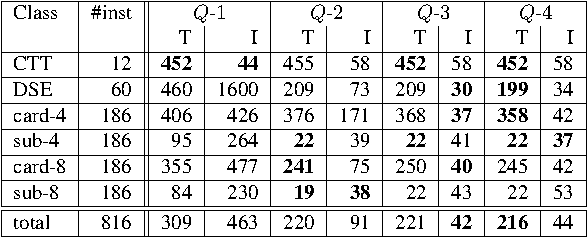
\includegraphics[width=\textwidth]{tables/query_comparison}
\caption{Comparison of different query techniques by runtime and number of solving calls}
\label{tab:query_comparison}
\end{table}

\begin{table}[H]
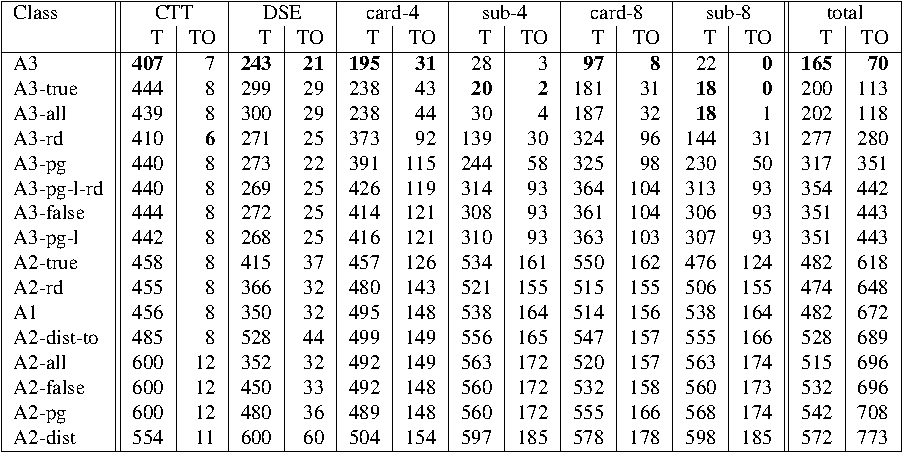
\includegraphics[width=\textwidth]{tables/time_comparison}
\caption{Comparison of approximation techniques by runtime and timeouts}
\label{tab:time_comparison}
\end{table}

\begin{table}[H]
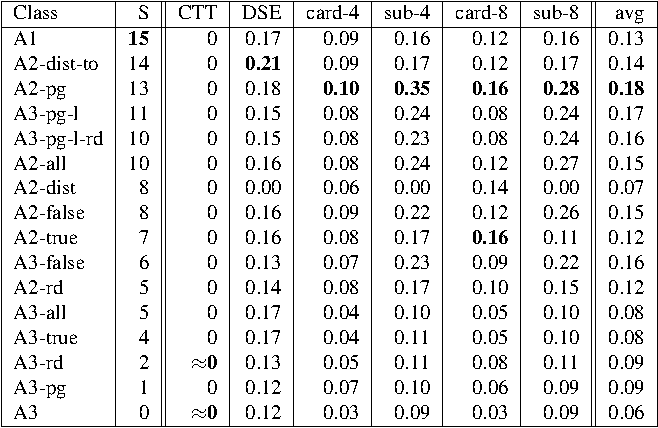
\includegraphics[width=\textwidth]{tables/diverse_comparison}
\caption{Comparison of approximation techniques by diversification quality}
\label{tab:diverse_comparison}
\end{table}

\begin{table}[H]
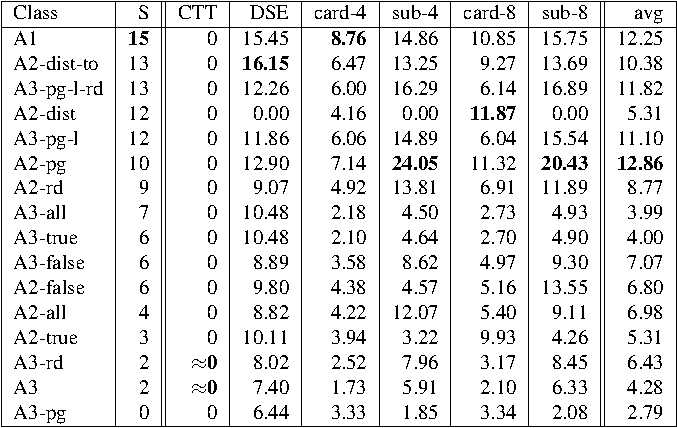
\includegraphics[width=\textwidth]{tables/min_dist_comparison}
\caption{Comparison of approximation techniques by minimum distance}
\label{tab:min_dist_comparison}
\end{table}
